\chapter{Case Study}\label{case_study}

This section presents a case study to assess the applicability of the proposed approach in the modeling of an application. The case study is based in
the Hotel Management System extracted from Jacobson{'}s work \cite{Jacobson:2004:ASD:1062430}. This example allows the modeling of important
aspect-oriented funcionalities and is consolidated in the literature. The use cases represented in this case study are the reservation of rooms,
handling of a waiting list of customers and the logging of messages. As we are not going into details about the modeling of the structure of
aspect-oriented software, the structural diagrams of the case study will not be show in this section, although they can be represented using the
stereotypes of the UML profile.

Sequence diagrams are used to represent the behavior of the core and crosscutting concerns, using the profile and the process proposed by this
approach. The modeling of concerns using behavioral diagrams gives subsidies to achieve the toogling of views, that allows better understanding of
aspect-oriented applications, visualizing the effect of the aspects in the system. We start with the sequence diagram of the reserve room concern,
that is show in figure \ref{fig:case_study_behavioral_reserve_room}. In a room reservatiom, if the room isn't available, an exception is raised in the
method \textit{updateAvailability()}, otherwise, the reservation is done and the customer receives a confirmation code.

  \begin{figure}[!b]
	\centering
	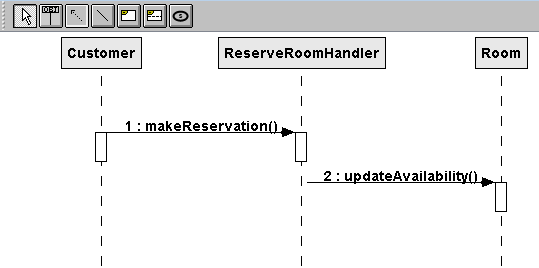
\includegraphics[scale=0.6]{img/case_study_behavioral_reserve_room.png}
	\caption{Advice behavior of the core concern to reserve a room.}\label{fig:case_study_behavioral_reserve_room}
  \end{figure}
  
The other concerns to be modeled are the crosscutting concerns that contains pointcuts and advices. The log concern needs to account the number of
requests to a room. To achieve this, we must define a pointcut that captures the calls to the \textit{Room} class. This pointcut is modeled using the
state machine diagram and is show in figure \ref{fig:case_study_behavioral_pointcut_log}. With the pointcut defined, we create the sequence diagram to
the log concern. The diagram is show in figure \ref{fig:case_study_behavioral_log} and contains as the first lifeline the \textit{LogAspect}.
Accordingly to the proposed approach, an aspect in the sequence diagram must have a state invariant associated, which is the trigger to execute the
sequence of messages. In this case, the state invariant \textit{RoomCall} is associated with the \textit{LogAspect} and points to a pointcut
previously defined in the state machine diagram. The semantics here is that the sequence of messages will execute only when the pointcut is satisfied.
The message to be executed when the pointcut is satisfied is a call to the method \textit{log()} of the \textit{Logger} class. It is important to be
aware of the advice type, that is defined as a tagged value in the state invariant. The tagged value is not being show in the sequence diagram to
not clutter the diagram. The proposed approach supports three types of advice types: before, after or around. In this case, the advice type is after,
which means that the log behavior will execute after any method call to the \textit{Room} class. The sequence diagram contains a combined fragment of 
type optional, that defines that the log only will be performed if the application is not frozen. An application is not frozen when it is running in the development environment.

  \begin{figure}[tb]
	\centering
	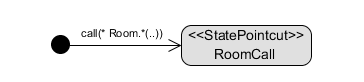
\includegraphics[scale=0.6]{img/case_study_behavioral_pointcut_log.png}
	\caption{Pointcut of the crosscutting concern to log messsages.}\label{fig:case_study_behavioral_pointcut_log}
  \end{figure}
  
  \begin{figure}[tb]
	\centering
	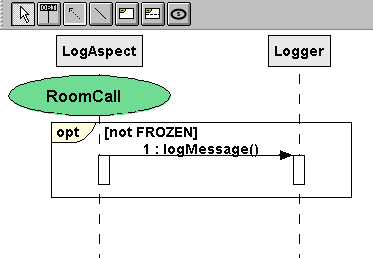
\includegraphics[scale=0.6]{img/case_study_behavioral_log.png}
	\caption{Advice behavior of the crosscutting concern to log messages.}\label{fig:case_study_behavioral_log}
  \end{figure}

The last concern to be modeled is the waiting list, that adds the customer to a waiting list when a room isn't available. To achieve this, we need a
pointcut that captures when a customer try to reserve a room without success, because it is unavailable. Figure
\ref{fig:case_study_behavioral_pointcut_waiting_list} shows a pointcut that captures calls to the method \textit{updateAvailability()} of the
\textit{Room} class, raising the \textit{NoRoomsAvailable} exception. Besides the pointcut definition, we need to define the behavior of how a
customer is added to the waiting list. This behavior is modeled in the sequence diagram of figure \ref{fig:case_study_behavioral_waiting_list}. The
diagram has the \textit{WaitingListAspect} as the first lifeline and has a sequence of messages to be executed when the system raises an exception
that no rooms are available. These messages will be executed after the exception raising, because the advice type of the state invariant is after.
Again, the tagged value is not being show in the sequence diagram to not clutter the diagram.

  \begin{figure}[tb]
	\centering
	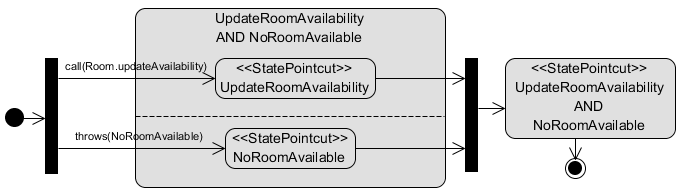
\includegraphics[scale=0.6]{img/case_study_behavioral_pointcut_waiting_list.png}
	\caption{Pointcut of the crosscutting concern to handle a waiting list.}\label{fig:case_study_behavioral_pointcut_waiting_list}
  \end{figure}
  
  \begin{figure}
	\centering
	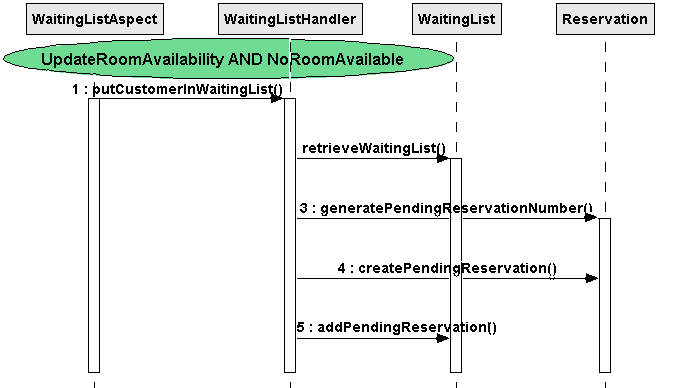
\includegraphics[scale=0.6]{img/case_study_behavioral_waiting_list.png}
	\caption{Advice behavior of the crosscutting concern to handle a waiting list.}\label{fig:case_study_behavioral_waiting_list}
  \end{figure}
  
   \begin{figure}
	\centering
	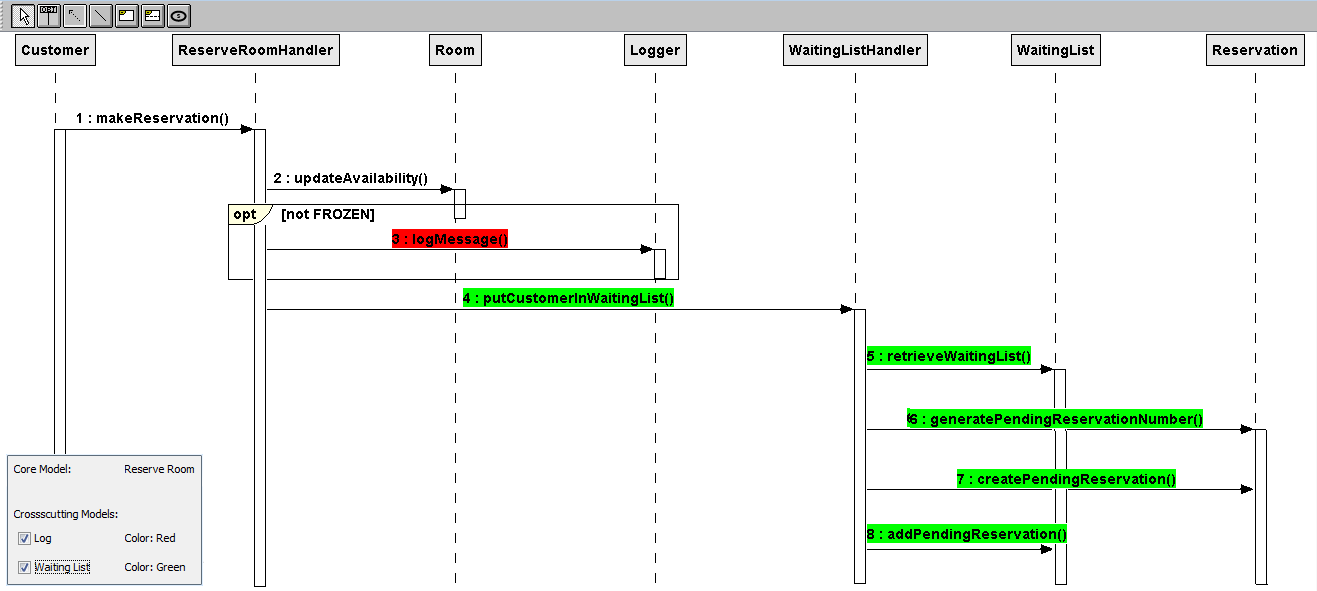
\includegraphics[scale=0.4]{img/case_study_compound_2.png}
	\caption{Case Study: Reserve
	Room composed with Log and Waiting List.}\label{fig:case_study_compound_2}
  \end{figure}
  
After the modeling of all the core and crosscutting concerns, the modeler may interchange the model views, selecting which concerns he wants to see
composed in the same diagram. The SEA/Aspect tool allows the selection of more than one model to be composed at the same time. Figure
\ref{fig:case_study_compound_2} shows a compound model, with the concerns of reserve room, log and waiting list composed together. The compound
diagram shows the model selector in it is right bottom, that allows changing the models that are being show. The messages of different concerns are
illustrated with different colors, as each concern has a color associated with it. This is useful to differentiate which messages comes from which
aspect in the compound model.